\chapter{Summary and additional work}\label{Future}
\section{Summary of contributions}
In chapter~\ref{introduction} this thesis explores the basic constructs of how animals interact in different types of swarms such as shoals of fish, murmurations of starlings, and ant colonies. The chapter examines how these biological swarms have been studied and modelled to produced autonomous multi-agent robotic systems. The evolution of swarming techniques from the early modelling and mimicking of the biological swarms has shown that metrics are needed to provide an understanding of how agent interactions change over time and how the swarming algorithms affect the resultant swarm structures.

The remainder of the section focuses on the major contributions of the research:

\begin{itemize}
\item Model/Simulator
\item Inter-agent magnitude metric/Swarm Types
\item Perimeter coordination
\item Concave Reduction
\item Flood filling
\end{itemize}

\subsection{Model/Simulator}
Earlier research has identified the use of field effects as being an effective method of modelling an agent's behaviour within a swarm. This has led to vector mathematics being the most prominent mathematical modelling tool in swarm theory. Field effect modelling through vector mathematics is discussed in chapter~\ref{chapter:methods}. This chapter also introduces a graduated field effect implementation for cohesion~(\autoref{sec:Cohesion1}) and repulsion~(\autoref{sec:Repulsion1}) this approach helps to reduce collisions. The model also applies an aggregate weighted model that allows the field effect algorithms to be tailored to create regular structures~(\autoref{methods:weightedModel}).

All of the experimental work in this thesis has been carried out using a simulator written specifically for this project. Chapter~\ref{chapter:simulator} discusses the simulation process and the object model used for the representation of the swarming agents. The chapter discusses the mathematical models that have been applied to the modelling. The chapter also discusses how the simulator is applied to the experiments and how the results are achieved. The simulator has been designed with a specific set of requirements for this thesis and it allows the modelled swarms to be analysed by creating aggregated simulation data sets. The datasets consist of each agent's \textit{inter-agent vector magnitudes}, inter-agent distances, and inter-agent relationships in the form of cohesion and repulsion vectors. The simulator is configurable in terms of allowing the weighted model and field effects defined in chapter~\ref{chapter:metric} to be visualised and allows the environmental parameters to be altered to achieve the required effects discussed throughout. The simulator, being based on an object model, has allowed two applications to be developed: a graphical setup environment to create simulation configurations and a command line based simulation tool to execute the experiments. The graphical tool is capable of running small simulations in a real-time mode but for large swarms a command line version is used which incorporates simulated time to ensure the accuracy of the simulation results. The simulator uses a discrete time model to capture and implement the models~(\autoref{sim:time}). 

\subsection{Inter-agent magnitude metric}
The application of swarms as a platform to solve problems has necessitated the need to understand how agents in a swarm can be distributed and how their movements can be coordinated efficiently. Chapter~\ref{chapter:metric} identifies the \textit{inter-agent vector magnitude} as being a suitable metric to measure a swarm's internal movements~(\autoref{section:MagnitudeDynamics}). 

%% \begin{figure}[H]
%% \begin{center}
%% 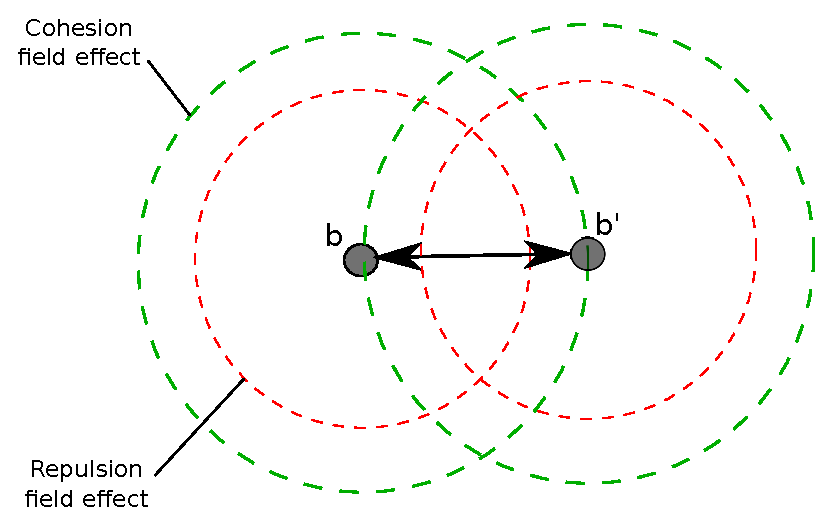
\includegraphics[width=9cm]{CHAPTER-9/figures/MagnitudeMetric1}
%% \end{center}
%% \caption{Magnitude Metric\label{additional:MagnitudeMetric1}}
%% \end{figure}

The chapter compares this new metric with the distance metric~(\autoref{section:DistanceDynamics}) currently in use and demonstrates how the \textit{inter-agent vector magnitude} is better suited to identifying the state of a swarm.  

%% \begin{figure}[H]
%% \begin{center}
%% 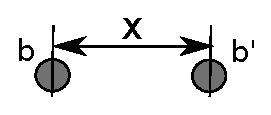
\includegraphics[width=3cm]{CHAPTER-9/figures/DistanceMetric1}
%% \end{center}
%% \caption{Distance metric\label{additional:DistanceMetric1}}
%% \end{figure}

The \textit{inter-agent vector} metric is based upon the component vectors that determine the inter-agent interactions rather than the resultant distribution of the agents. This change of focus creates a transferable metric that allows the effect of any field effect based algorithm to be analysed independently of the resultant distributions that the field effects create. The new metric also allows the `hidden potential' of a swarm to be identified. Inter-agent distance distribution does not show the underlying `potential' with respect to an agent's current vector magnitude state. The new metric allows a swarm to be identified as being in a repulsive state such that it will expand over time or as being in a cohesive state which results in the swarm remaining a single entity with a tendency to `stick' together. The application and benefits of the new metric are discussed further in~\autoref{additional:MoreWork}.

In chapter~\ref{chapter:SwarmType} the effect of varying the field effects of a swarm's agents and the impact this has on the swarm's structure is examined. The chapter demonstrates how the field effects can be used to produce different types of swarms based upon inter-agent `visibility'. The chapter demonstrates how the swarm models can be analysed using both the distance metric and the new \textit{inter-agent vector metric} defined in chapter~\ref{chapter:metric}. The chapter demonstrates how identifying the underlying inter-agent interactions allows the type of swarm to be identified and also highlights improvements that can be made in the field effects model to improve a swarm's structure. 

\subsection{Perimeter coordination}
If the application of a swarm requires it to move in a specific direction then an additional attribute must be added to the field effect model to create a goal based characteristic. In chapter~\ref{chapter:coordination} alternative swarm co-ordination algorithms are presented to create goal-based swarms capable of being applied to reconnaissance type tasks. The alternate methods are compared to a baseline static swarm to identify the effects the algorithms have upon a swarm's structure. The comparisons are carried out using both the distance-based metric and the new \textit{inter-agent vector magnitude} metric. This thesis explores three basic approaches to implementing a goal based characteristic. All agents using their GPS modules, only perimeter based agents using their GPS modules, and finally using a subset of the perimeter selected using a simple counting technique. The findings in this chapter are that by reducing the number of coordinator agents in a swarm it is possible to maintain a stable internal structure whilst imposing a directional bias to a swarm. The most effective technique is to use the smallest subset of the perimeter by using the basic count algorithm~(\autoref{section:stabilityComparison1}). The algorithm that produced the most internal disturbance is the `all agents' algorithm where all agents are coordinators. The chapter also examines the effects of balancing the field effects on a pro-rata basis (number of coordinators) to reduce the negative effects the algorithms can introduce. This is achieved by adjusting the individual vector component weightings for each of the algorithms used~(\autoref{sec:AlternateBias1}). When the \textit{weighting movement direction} parameters are altered the basic count mechanism is still the most effective algorithm~(\autoref{fig:BaselineAllMag100-60-20-2}).

\subsection{Concave reduction}
Chapter~\ref{chapter:ConcaveReduction} examines how swarms can exhibit emergent behaviours from a simple algorithm. A localised algorithm is used to improve inter-agent distributions by identifying gaps between an agent's neighbours and moving the agent towards the gap. This simple change to the swarming model produces two behavioural changes. It causes a swarm to close voids and migrate towards a more uniform shape. These effects can be interpreted as a `healing' effect as they cause the swarm to be more uniform in shape with no internal anomalies. This can be useful when a swarm's structure is disrupted by a failed agent or from disruptions to a swarm's path. This behaviour can also be applied to encapsulating an object. The object encapsulation effect is presented in terms of an existing application area in the petrochemical industry where they have identified the use of swarms as a potential method of controlling oil spillages~(\autoref{voids:ObjectSurrounding}). The technique used in this thesis uses a Boid-based swarming approach which differs to the current research which uses an ant-colony-based approach. This `healing' behaviour is also applied to goal-based swarms in an attempt to remove voids in a reconnaissance based swarm when a swarm's path is disrupted~(\autoref{concave:mobileSwarm1}). The thesis demonstrates that the emergent behaviour is able to remove a void created by an obstacle improving the coverage of the swarm's path using the \textit{concave-reduction} effect.

\subsection{Flood filling}
In chapter~\ref{chapter:flooding} the cohesion and repulsion field effects (\textit{interaction vectors}) are used to create an area filling behaviour using a swarm of a fixed size. This is achieved by increasing the repulsion field effect of the agents to influence the distribution of the agents such that the agents fill a bounded area. The chapter examines two different techniques of coordinating the expansion process. The first technique involves using a `normal' swarm that utilises both cohesion and repulsion to create a swarm that acts as a single entity and ensures agents maintain `visibility' of each of its neighbours. The second technique exploits the fact that the swarm is in a bounded area and removes the cohesion field effect and uses only the repulsion field to expand the agents throughout the space. The metrics discussed in chapter~\ref{chapter:metric} are used to identify the effects of the expansion on the swarms internal structures and to identify terminating conditions for the filling behaviours.

\section{Additional work}\label{additional:MoreWork}
The research in this thesis has investigated several issues with respect to swarm analysis but has also raised further questions that need to be answered. The new metric allows swarms to be analysed in a completely different way and has opened up the possibility of analysing new swarm configurations.

\subsection{Metric comparison}\label{additional:fieldsWork}
Swarms are often constructed from heterogeneous agents that adapt to stimuli but the agents themselves are usually modelled using homogeneous field effects. This modelling of homogeneous field effects lends itself to being measured and monitored by a distance based metric as defined by Navarro et al. \cite{NIM:09} due to the regular shapes and structures that emerge. The dependence on regularity of shapes and structures is a limitation of the distance metric due to the aggregation of the distances not reflecting the mathematical model that creates the structures. The magnitude based metric overcomes that limitation by analysing the vectors that effect the agent distribution. With heterogeneous field effects the inter-agent distances will be varied in an equilibrium state due to the way the field effects overlap when agents interact. 

The \textit{inter-agent vector magnitude} metric takes into consideration the resultant effects of the mathematical model~\autoref{additional:FieldEffects} rather than just arbitrary distances between agents. Preliminary tests have shown that the metric is able to provide meaningful results for agents that use varying field effects within the same swarm structure. The distance metric is unable to achieve this analysis due to the distances being a physical presentation of the mathematical model. The balancing of \textit{interaction vectors} affect the resultant agent distributions. Distance variance is different to magnitude variance even though with a homogeneous agent they appear to be similar as shown by the metric comparison. \autoref{additional:FieldEffects} shows a swarm construct where the interaction of the agents would be unidirectional, agent $b$ is affected by agent $b'$ with respect to cohesion but agent $b'$ is not affected by $b$. This type of interaction does not produce a meaningful distance metric as there is no distinction between agents with different field effects producing the different agent distributions.  

\begin{figure}[H]
\begin{center}
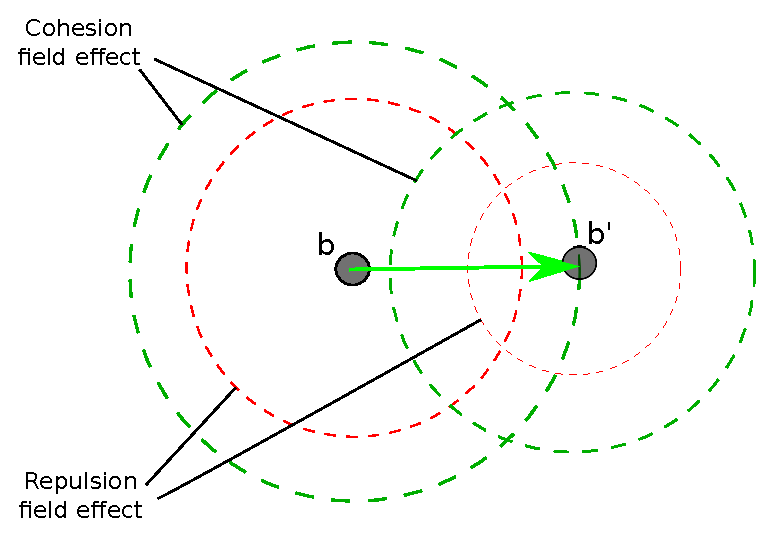
\includegraphics[width=9cm]{CHAPTER-9/figures/FieldEffects}
\end{center}
\caption{Varied field effects\label{additional:FieldEffects}}
\end{figure}

Further work needs to be carried out to identify how variations in field effects affect the overall structure of a swarm which would be more realistic when transferred to the real world as sensors rarely provide consistent results. Physical environments have conditions that may affect sensor readings i.e. an omni-directional camera will be affected by visibility. There is also the possibility of agents having different techniques of implementing the cohesion and repulsion models, this could improve a swarm's performance in specific applications. This is similar to how ant colonies use different casts with a swarm to create efficiencies in their activities such as foraging for resources. This combination of using a Boid-based swarm with a cast system based on field effects measured by the \textit{inter-agent vector} metric opens up a new method of modelling and analysing a swarm. This thesis has used a graduated cohesion effect however other methods of applying cohesion such as using a fixed vector could be applied or a mixture depending upon environmental conditions. These changes would affect the results from the distance based metric but the mixed implementations can be analysed by the new \textit{inter-agent vector} metric.

\autoref{additional:FieldEffects2} shows a more complex situation that can occur in a heterogeneous field effect swarm. In this scenario 2 sets of agents have different field ranges ($b,b^{'}$ and $b^{''},b^{'''}$). The use of the distance metric in this environment would not be applicable due to variation in the distances that the different field effects create. The \textit{inter-agent vector} metric defined in this thesis would allow an analysis of the environment due to balancing of the field effects resulting in vectors that will have equivalent resultant magnitudes.

\begin{figure}[H]
\begin{center}
\includegraphics[width=9cm]{CHAPTER-9/figures/FieldEffects2}
\end{center}
\caption{Complex swarm interactions\label{additional:FieldEffects2}}
\end{figure}

The additional work required here would be to identify potential applications of these variations in the field effects that could improve existing swarm applications. For example, if an agent is on a perimeter would the swarm benefit from reducing the field effects to create a greater compression effect? Would having a mixed field effect swarm produce better coverage of an area? What would be the impact of having variable field effects upon a goal-based swarm?

\subsection{Area flooding}
In chapter~\ref{chapter:flooding} the ability of a swarm to fill a space was examined using the distance and \textit{inter-agent vector} metrics. The swarms that were applied to the task used homogeneous field effects. If agents could vary their field effects based on their position in a swarm (e.g. agents at the boundary) it may be possible to improve coverage. As a swarm expands it was found that the expansion process was affected by the distribution of the agents on convex and concave corners~(\autoref{additional:FloodEdges1}). If agents were able to vary the effect based on detected features the swarm may be able to achieve set goals more efficiently (use less energy) and effectively (reducing time). Confined spaces may have narrow paths linking larger chambers and allowing agents to change their field effects may allow a swarm to propagate through this type of environment more effectively. 

\begin{figure}[H]
\begin{center}
\includegraphics[width=6cm]{CHAPTER-9/figures/FloodEdges1}
\end{center}
\caption{Flood fill edges\label{additional:FloodEdges1}}
\end{figure}

Additional experiments need to be developed to identify why the corners and edges caused these problems and also to test the affect of using alternate field effects. One of the possible areas of research here would be to identify if there is a correlation between the field effect size and the angle of any boundary anomalies.
 
\subsection{Directional shape forming}\label{sec:DirectionalShape1}
The \textit{destination vector} as discussed in~\autoref{sec:Direction1} has been based upon a swarm having a fixed single destination however this model can be changed slightly to produce two more possible swarming effects by applying the \textit{destination vector} to a set of points. The effects that are possible from these simple changes are to create swarms that create arbitrary shapes or a swarm that will migrate along a specific path. The \textit{destination vector} required to achieve these two emergent behaviours can be implemented using the coordination techniques discussed in chapter~\ref{chapter:coordination}.

Shape forming~\cite{EP:07} and path following (which is an enhancement to the shape forming) in swarms is caused by the coalescence of the agents towards a point (target) when attempting to ensure the swarm exists as a single entity. The target is identified by the coordinator's \textit{destination vector} being towards the closest destination. Due to the cohesive properties of a Boid-based swarm a large swarm will therefore coordinate the centroid towards the target.

\subsubsection{Shape forming swarms}\label{sec:DirectionalShape3}
For shape forming to take place the distance between the destination points must be less than half of the radius of the swarm for the coordinators destinations to change as the swarm migrates towards the first destination point. This process will continue as the swarm `spreads' over the set of destination points. This is shown in~\autoref{methods:SwarmShape}.

$v_d(b)$~(\autoref{eq:Destination2}) is the resultant \textit{destination vector} where $D$ is the set of all possible destinations. $b$ is the agent's current position and $min(b,D)$ returns the destination which has the smallest magnitude in relation to agent $b$. $F(.)$ returns a vector from agent $b$ position to the nearest destination.

\begin{center}
\begin{equation}\label{eq:Destination2}‎
v_{d}(b) =‎ F(b,min(b,D))
\end{equation}‎
\end{center}

Figure~\autoref{emerge:Shaping1} shows the swarm initially encountering the set of destination points. As the simulation continues the proximity of the destination points influences different coordinator agents and the swarm is `pulled' by the coordinators around the set of destinations. Figure~\autoref{emerge:Shaping4}~shows the resultant swarm distributed around the set of points. The effect emerges due to the coordinator agents `exerting' a compression effect based on different points this combined with the swarms cohesive bias holding the swarm together and the destination vectors for the agents deform the swarm to an equilibrium point forming the shape.

\begin{figure}[H]
\centering
\subfigure[Stage 1]{
	 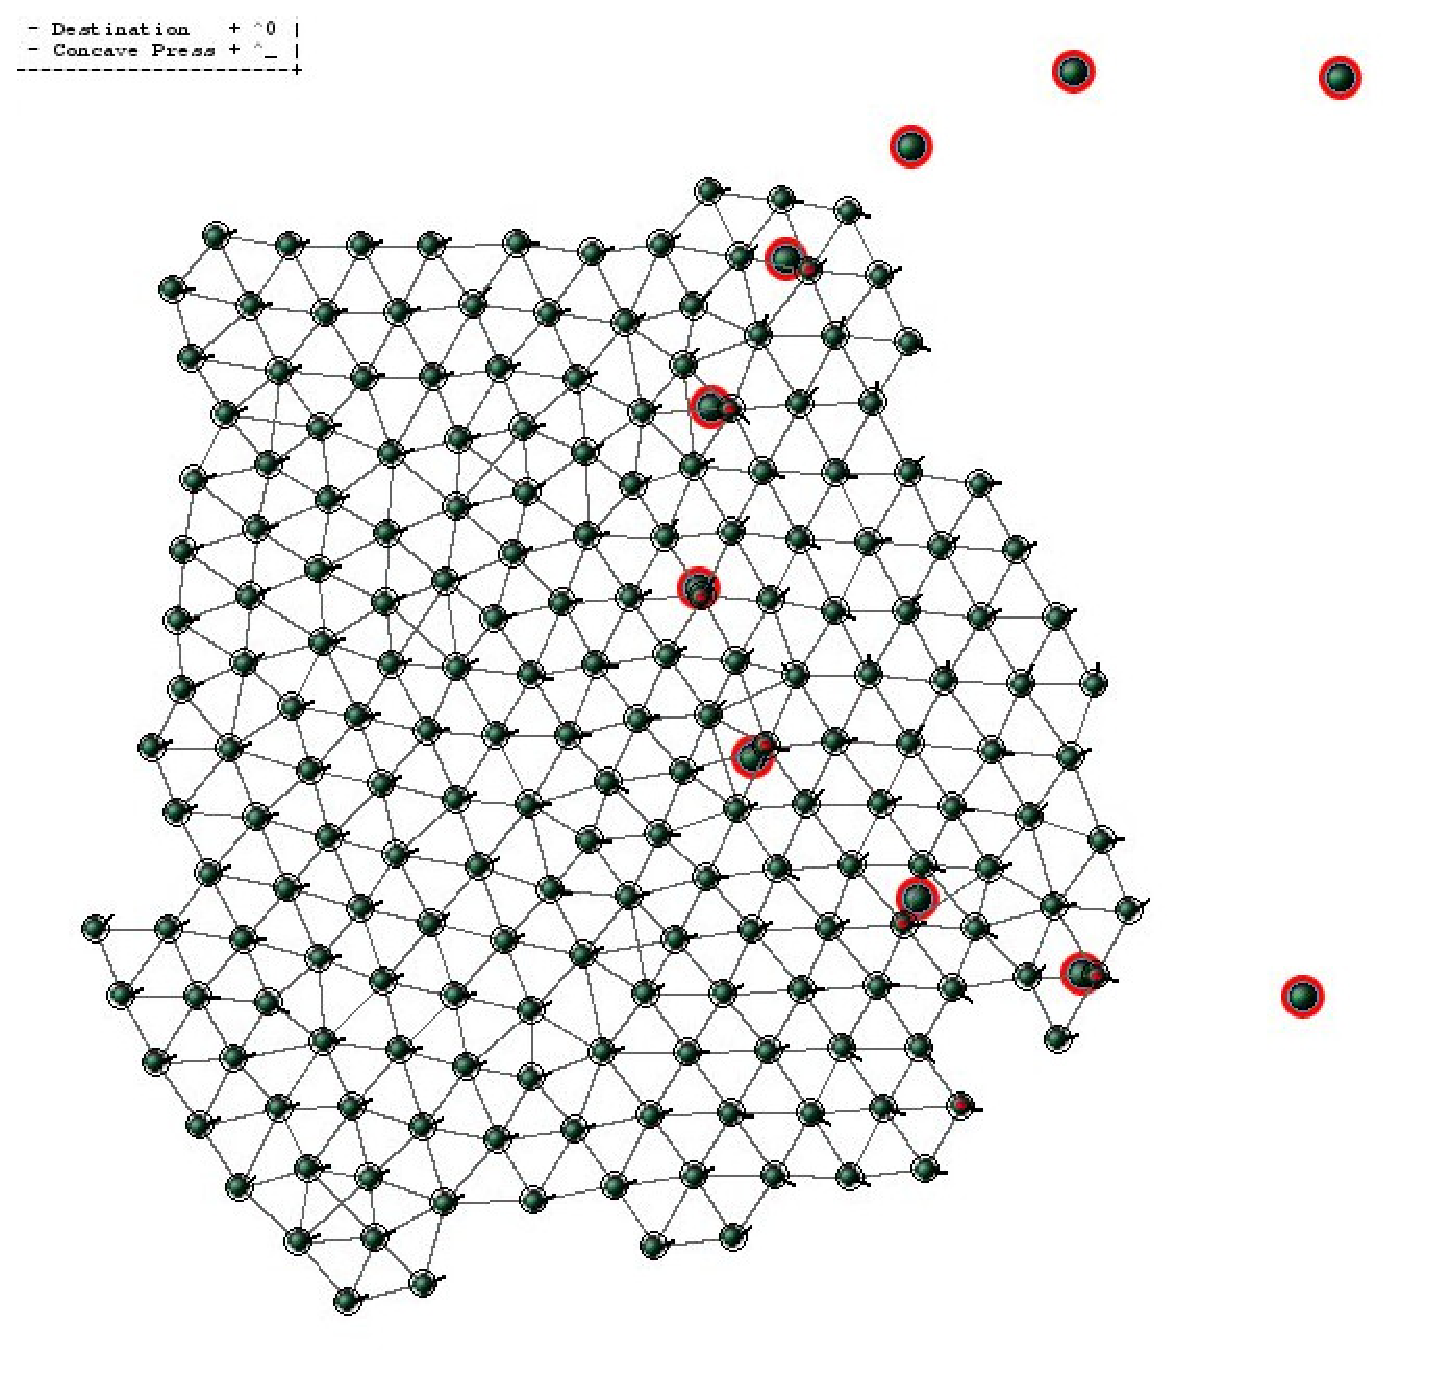
\includegraphics[width=4cm]{CHAPTER-9/figures/SwarmShaping1}
	 \label{emerge:Shaping1}
}
\subfigure[Stage 2]{
	 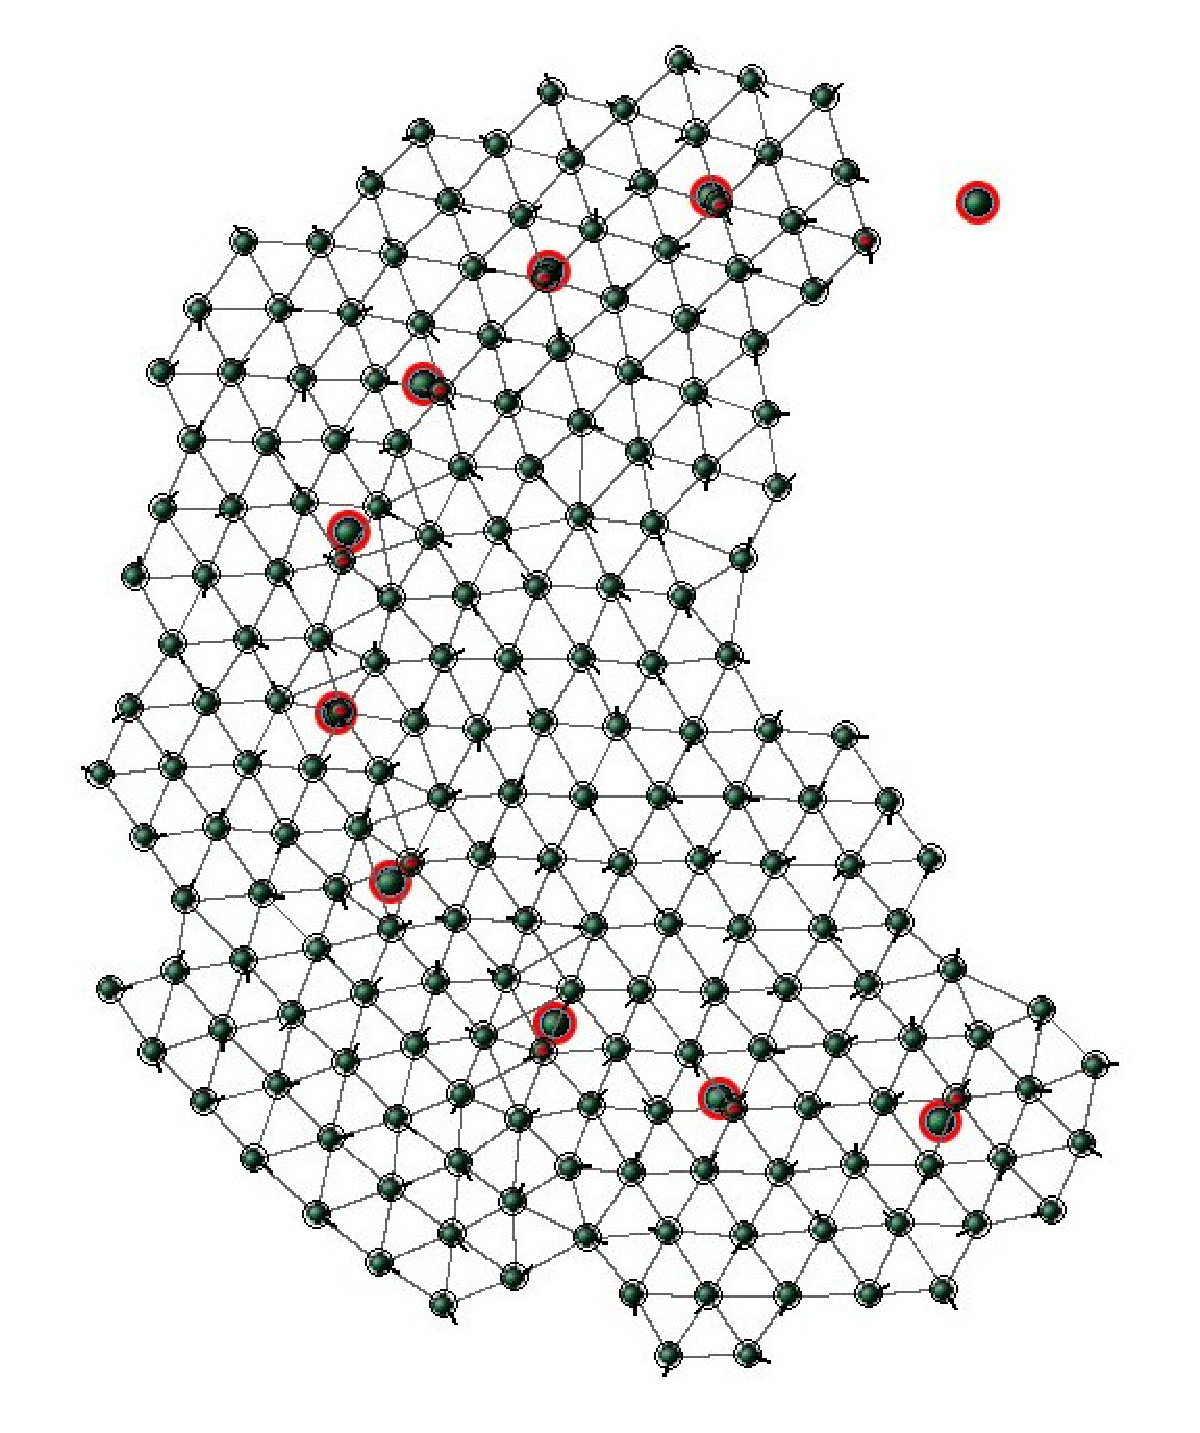
\includegraphics[width=4cm]{CHAPTER-9/figures/SwarmShaping2}
	 \label{emerge:Shaping2}
}
\subfigure[Stage 3]{
	 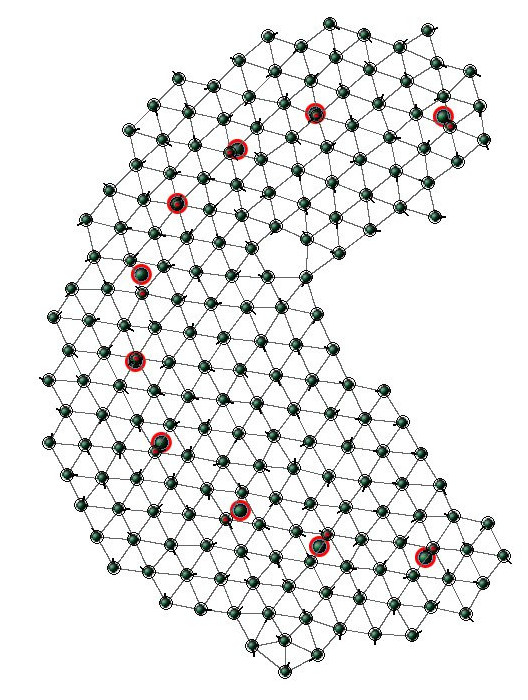
\includegraphics[width=4cm]{CHAPTER-9/figures/SwarmShaping4}
	 \label{emerge:Shaping4}
}
\caption{Boid based swarm shaping}
\label{methods:SwarmShape}
\end{figure}

Within this type of swarming effect there is a natural `self-healing' property~\cite{RS:08, KY:10} as having a destination will naturally cause a swarm's centroid to coalesce around a single point which will therefore create a compressing effect. Non directional swarms and swarms that have distant goals do not naturally exhibit this behaviour, however it can be induced as discussed in chapter~\ref{chapter:ConcaveReduction}. 

\subsubsection{Path following swarms}\label{sec:DirectionalShape4}
If the destination set is a path that must be followed then a slight change is required to the logic used within the shape forming algorithm. When a coordinator agent falls within a specified range of a destination it can be classed as having successfully met a target. The agent can then move to the next destination in the set. This will cause the agents \textit{destination vector} to move causing the non-coordinator agents to follow through due to the proximity cohesion effect. This effect cascades through all the coordinators and the swarm will propagate along the set of destinations and therefore follow a predetermined trail.

\begin{figure}[H]
\centering
\subfigure[Stage 1]{
	 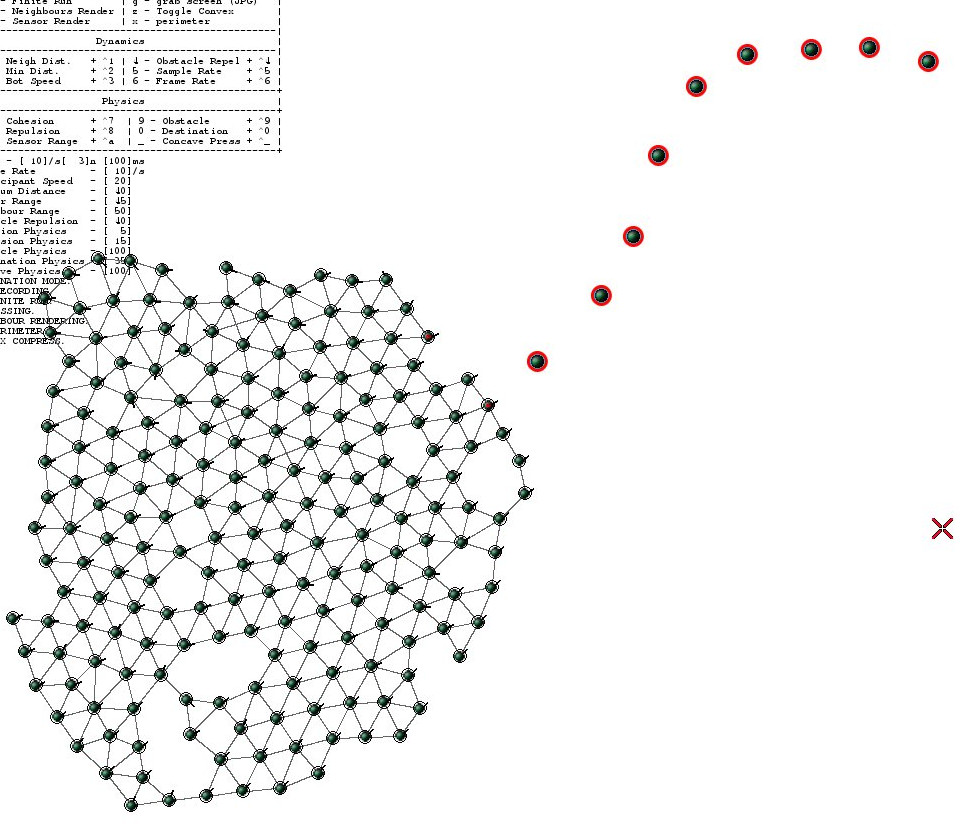
\includegraphics[width=4cm]{CHAPTER-9/figures/SwarmPath1}
	 \label{emerge:Path1}
}
\subfigure[Stage 2]{
	 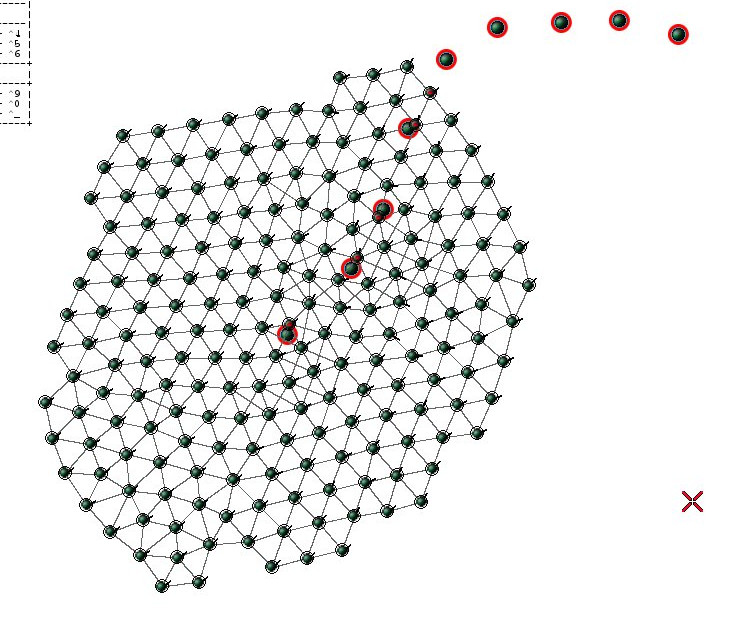
\includegraphics[width=4cm]{CHAPTER-9/figures/SwarmPath2}
	 \label{emerge:Path2}
}	 
\subfigure[Stage 3]{
	 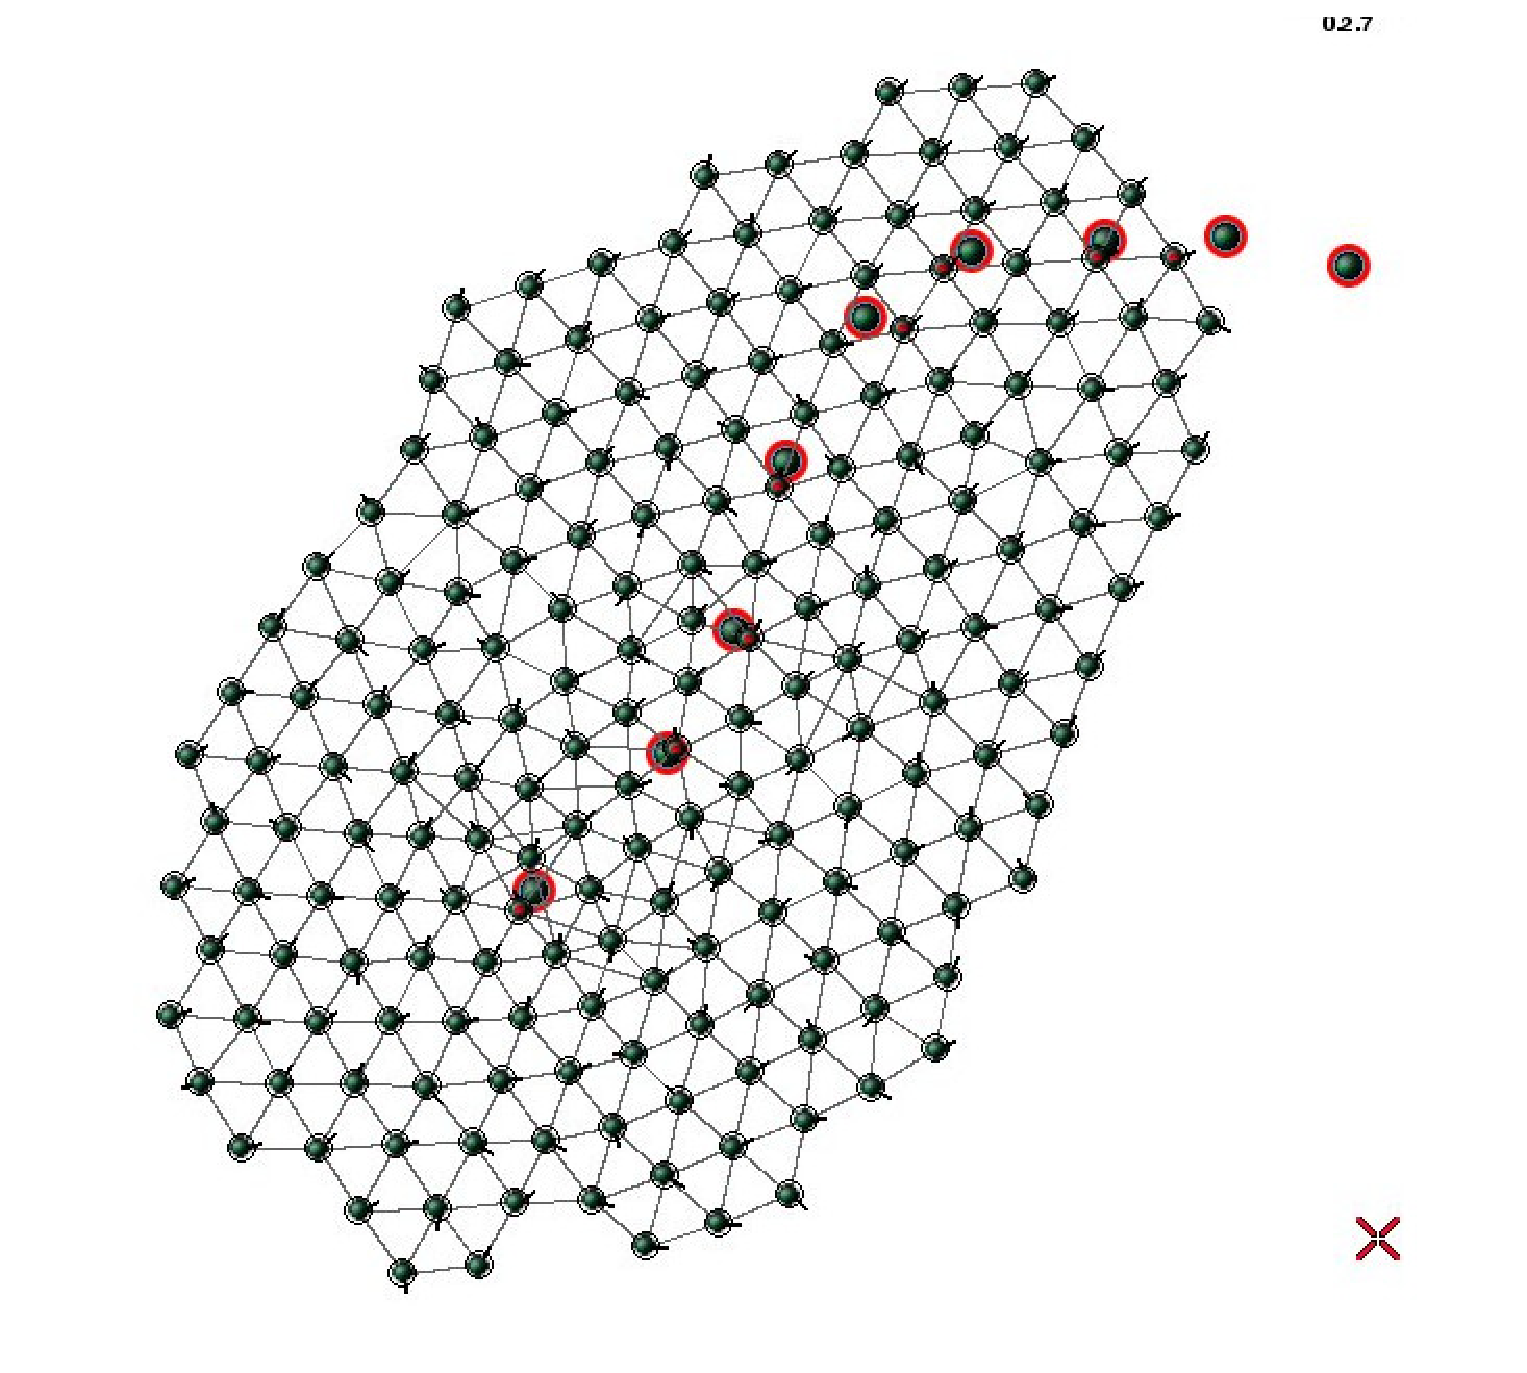
\includegraphics[width=4cm]{CHAPTER-9/figures/SwarmPath3}
	 \label{emerge:Path3}
}
\caption{Boid based swarm path following}
\label{methods:SwarmPath}
\end{figure}

\autoref{methods:SwarmPath} shows the effect in the stages of path propagation. Initially the whole swarm will be coordinated towards the nearest destination~(Figure~\autoref{emerge:Path1}). The leading edge of the swarm will then move onto the next destination drawing the swarm along~Figure~\autoref{emerge:Path2}. As each `goal' is met the swarm will move along the destination points~Figure~\autoref{emerge:Path3} and will eventually result in the swarm centering on the final destination point.

\subsection{Simulator enhancements}
All of the additional work detailed above will require the simulator to be developed further to allow additional modelling to be carried out. Several aspects of the current simulator are geared towards modelling homogeneous agents rather than each agent having an individual configuration, however the object model supports the required features in its current form. The object model used to develop the simulator already supports the generic modelling requirements for the future work but they are not fully exploited by the current implementation of the applications. i.e. all agent object instances hold their own field effect values that are globally adjusted within the software.

The additional work will require further adaptations to the bespoke simulation software to generate the new behaviours identified above and to allow for the additional data logging requirements.
